% !TEX program = xelatex
\documentclass[11pt, a4paper]{ctexart}

% ========== 宏包 ==========
\usepackage[top=2cm, bottom=2cm, left=2.5cm, right=2cm]{geometry}
\usepackage{amsmath, amssymb}
\usepackage{graphicx}
\usepackage{booktabs}
\usepackage{array}
\usepackage{hyperref}
\usepackage{xcolor}
\usepackage{listings}
\usepackage{caption}
\usepackage{enumitem}
\usepackage{fancyhdr}
\usepackage{cite}
\usepackage{float}

% ========== 紧凑间距 ==========
\setlength{\parskip}{0.3em plus 0.1em minus 0.1em}
\setlength{\abovedisplayskip}{6pt}
\setlength{\belowdisplayskip}{6pt}
\setlength{\floatsep}{8pt}
\setlength{\textfloatsep}{8pt}
\captionsetup{font=small, skip=4pt}

% ========== 超链接样式 ==========
\hypersetup{
    colorlinks=true,
    linkcolor=black,
    citecolor=blue!70!black,
    urlcolor=blue!60!black
}

% ========== 代码样式 ==========
\lstset{
    basicstyle=\small\ttfamily,
    backgroundcolor=\color{gray!8},
    frame=single,
    framerule=0.4pt,
    rulecolor=\color{gray!40},
    xleftmargin=1.5em,
    xrightmargin=0.5em,
    aboveskip=0.5em,
    belowskip=0.5em,
    breaklines=true,
    columns=flexible,
}

% ========== 页眉页脚 ==========
\pagestyle{fancy}
\fancyhf{}
\fancyhead[R]{\small 基于 CLIP 的 ABO 商品图文检索实验报告}
\fancyfoot[C]{\thepage}
\renewcommand{\headrulewidth}{0.4pt}

% ========== 标题格式 ==========
\usepackage{titlesec}
\titlespacing*{\section}{0pt}{1.2em}{0.5em}
\titlespacing*{\subsection}{0pt}{0.8em}{0.3em}

% ========== 文档信息 ==========
\title{\vspace{-1.5cm}\textbf{基于 CLIP 的 ABO 电商商品图文检索实验报告}}
\author{[待填写] \quad 课程：程序设计语言 \quad 2026 春季学期 \quad 小组成员与分工：[待填写]}
\date{}

\begin{document}
\maketitle
\thispagestyle{fancy}

% ========== 摘要 ==========
\begin{abstract}
\noindent
本报告围绕电商场景中的商品图文检索任务，基于 Amazon Berkeley Objects (ABO) 商品数据集构建了一个以 CLIP 为核心的 text-to-image 检索系统。实验选取 14 个商品类别，每类 400 张图片，共 5600 条样本，并按类别均衡划分为训练集 4480 条、测试集 1120 条。模型方面，本文比较了三类方法：原始预训练 CLIP、冻结 CLIP 编码器并训练输出投影层的 Linear Probe，以及在 CLIP Transformer 后部模块中注入低秩适配器的 LoRA 微调模型。

\medskip\noindent
为研究文本描述细粒度对检索性能的影响，本文构造了五类 prompt：\texttt{type}、\texttt{material}、\texttt{brand}、\texttt{brand\_material} 和 \texttt{full}。实验采用 \texttt{Recall@K}、\texttt{MRR@K} 和 \texttt{NDCG@K} 作为评价指标，并分别报告 $K=5,10,20$ 的结果。实验结果显示，完整商品标题 prompt 显著优于较粗粒度 prompt；在 \texttt{full} prompt 下，LoRA 模型取得最佳性能，\texttt{Recall@5} 达到 $0.8339$，相比原始 CLIP 的 $0.5446$ 提升 $0.2893$。

\medskip\noindent
\textbf{关键词：} CLIP；ABO 数据集；电商商品检索；Prompt 细粒度；Linear Probe；LoRA
\end{abstract}

\section{问题背景与研究目标}

随着电商平台商品规模持续增长，用户越来越依赖自然语言描述进行商品搜索。传统检索方法往往依赖人工标签或关键词匹配，难以充分理解商品图片与文本描述之间的语义对应关系。CLIP 通过大规模图文对比学习获得了较强的跨模态表征能力，但直接应用于细粒度商品检索时，仍会受到商品类别、品牌、材质、标题描述粒度等因素影响。

本实验希望回答以下问题：
\begin{enumerate}[leftmargin=2em, itemsep=0pt]
    \item 原始 CLIP 在 ABO 商品图文检索任务中的基础表现如何；
    \item 轻量微调方法是否能提升商品 text-to-image 检索性能；
    \item 不同细粒度 prompt 对检索结果的影响有多大；
    \item 在 Top-5、Top-10、Top-20 等不同候选规模下，各模型性能是否保持一致趋势。
\end{enumerate}

\section{任务定义与整体思路}

\textbf{任务定义：} 给定一个商品文本 prompt，在候选商品图片库中检索与该文本最匹配的图片。本文主要评测 text-to-image 方向，即文本查询到图片返回的检索任务。

\textbf{整体思路：} 首先使用 CLIP \texttt{ViT-B/32} 提取图片和文本特征；然后将测试集图片向量写入 ChromaDB 向量数据库；评测阶段将每个商品的不同 prompt 编码为文本向量，并在图片向量库中检索 Top-K 候选。训练阶段分别使用 Linear Probe 和 LoRA 两种轻量微调方法，使商品图片与 \texttt{full} prompt 在向量空间中更加接近。

\section{数据集与预处理}

\subsection{数据来源与字段结构}

实验数据位于 \texttt{version2/data\_abo\_subset\_selected14\_english/}。核心文件 \texttt{abo\_subset.csv} 包含如下字段：
\begin{center}
\small
\texttt{ProductId, ItemId, Brand, Category, ProductType, Colour, Material, ProductTitle, Image, ImageURL, MainImageId}
\end{center}

数据集共 5600 条记录，\texttt{ProductId}、\texttt{ItemId}、\texttt{ProductTitle} 和 \texttt{Image} 均为唯一值，核心字段缺失率为 $0$。本实验选取 14 个商品类别，每个类别 400 条样本，类别分布完全均衡。

\begin{table}[H]
    \centering
    \caption{ABO 子集基本统计}
    \label{tab:dataset-stat}
    \begin{tabular}{lc}
        \toprule
        \textbf{项目} & \textbf{数值} \\
        \midrule
        样本总数 & 5600 \\
        训练集样本数 & 4480 \\
        测试集样本数 & 1120 \\
        商品类别数 & 14 \\
        每类样本数 & 400 \\
        品牌数 & 72 \\
        材质取值数 & 559 \\
        标题唯一数 & 5600 \\
        核心字段缺失率 & 0.0000 \\
        \bottomrule
    \end{tabular}
\end{table}

\subsection{数据划分}

为保持训练集和测试集类别分布一致，本文沿用原项目的分层切分思想：先按商品类别分别收集 \texttt{ProductId}，在每个类别内部使用固定随机种子打乱，再按 $8:2$ 比例划分训练和测试样本。由于每类均有 400 条样本，因此每个类别划分为 320 条训练样本和 80 条测试样本。

\subsection{Prompt 构造}

原始 Fashion 实验中主要比较简单 prompt 和详细 prompt。迁移到 ABO 数据集后，本文将 prompt 扩展为五种细粒度：
\begin{table}[H]
    \centering
    \caption{五种 prompt 细粒度设计}
    \label{tab:prompt-design}
    \begin{tabular}{lll}
        \toprule
        \textbf{Prompt 类型} & \textbf{模板} & \textbf{信息粒度} \\
        \midrule
        \texttt{type} & \texttt{a photo of a \{product\_type\}} & 商品类别 \\
        \texttt{material} & \texttt{a photo of a \{material\} \{product\_type\}} & 材质 + 类别 \\
        \texttt{brand} & \texttt{a photo of a \{brand\} \{product\_type\}} & 品牌 + 类别 \\
        \texttt{brand\_material} & \texttt{a photo of a \{brand\} \{material\} \{product\_type\}} & 品牌 + 材质 + 类别 \\
        \texttt{full} & \texttt{a photo of a \{product\_title\}} & 完整商品标题 \\
        \bottomrule
    \end{tabular}
\end{table}

由于 \texttt{Colour} 字段中存在较多 \texttt{Unknown Color}、\texttt{Multi}、\texttt{Multicolor} 等不稳定取值，本文最终未将颜色字段纳入 prompt 拼接，以降低噪声。

\section{模型设计与实现}

\subsection{原始 CLIP 模型}

CLIP 由图像编码器和文本编码器两部分组成，其核心思想是通过大规模图文对比学习，将语义匹配的图像和文本映射到同一个向量空间中，并使二者的表示尽可能接近。在文本分支中，CLIP 使用 Transformer 对输入 prompt 的 token 序列进行上下文建模，并取序列中的全局表示作为文本特征；在图像分支中，本文采用的 \texttt{ViT-B/32} 版本使用 Vision Transformer，将输入图像划分为固定大小的 patch，再将这些 patch 展平并映射为视觉 token，从而建模图像的全局语义信息。

设图像样本 $\{I_i\}_{i=1}^{N}$ 和文本样本 $\{T_i\}_{i=1}^{N}$ 分别经过图像编码器 $f_v(\cdot)$ 与文本编码器 $f_t(\cdot)$ 后得到特征表示。为了使用余弦相似度进行跨模态匹配，编码后的向量需要进行 $L_2$ 归一化：
\begin{equation}
    \hat{\mathbf{v}}_i = \frac{f_v(I_i)}{\|f_v(I_i)\|_2}, \qquad
    \hat{\mathbf{t}}_i = \frac{f_t(T_i)}{\|f_t(T_i)\|_2}
\end{equation}

归一化后的图像特征和文本特征通过点积计算相似度矩阵：
\begin{equation}
    S_{ij}=\hat{\mathbf{v}}_i^\top \hat{\mathbf{t}}_j
\end{equation}
其中 $S_{ij}$ 表示第 $i$ 张图像与第 $j$ 条文本之间的语义相似度。原始 CLIP 在本实验中不更新任何参数，直接作为零样本检索 baseline，用于衡量预训练模型在 ABO 商品域上的基础表现。

\begin{figure}[H]
    \centering
    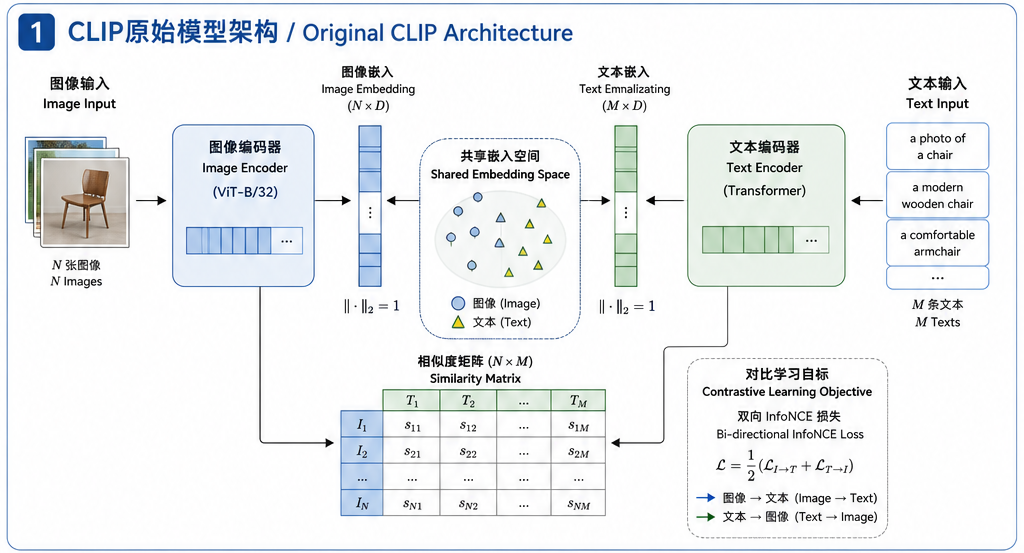
\includegraphics[width=0.72\textwidth]{assets/report_figures/clip原始架构图.png}
    \caption{原始 CLIP 模型结构}
    \label{fig:clip-original}
\end{figure}

\subsection{Linear Probe 微调}

Linear Probe 是一种轻量级微调方法。与全参数微调不同，该方法冻结 CLIP 原有的图像编码器和文本编码器，只在两端输出特征之后加入可训练的线性投影层。这样既能保留 CLIP 已有的通用视觉语言知识，又能通过少量参数适配 ABO 商品检索任务。本文的 Linear Probe 同时在图像侧和文本侧加入线性映射：
\begin{equation}
    \mathbf{z}_i^{(v)} = W_v \mathbf{v}_i + b_v, \qquad
    \mathbf{z}_i^{(t)} = W_t \mathbf{t}_i + b_t
\end{equation}

其中 $W_v,b_v$ 为图像侧投影层参数，$W_t,b_t$ 为文本侧投影层参数。投影后的图像和文本向量再次进行 $L_2$ 归一化，并使用双向 InfoNCE 损失进行训练：
\begin{equation}
    \mathcal{L} = \frac{1}{2}\left(
    -\frac{1}{N}\sum_i \log \frac{\exp(\tilde{S}_{ii}/\tau)}{\sum_j \exp(\tilde{S}_{ij}/\tau)}
    -\frac{1}{N}\sum_i \log \frac{\exp(\tilde{S}_{ii}/\tau)}{\sum_j \exp(\tilde{S}_{ji}/\tau)}
    \right)
\end{equation}

其中 $\tau$ 为温度系数。该损失同时约束 ``图像到文本'' 和 ``文本到图像'' 两个方向，使同一 batch 内匹配的图文对相似度更高、不匹配的图文对相似度更低。由于原始 CLIP 与 LoRA 模型的输出维度均为 512，为保证不同模型之间的评估结果具有可比性，本文将 Linear Probe 的投影维度也固定为 512。

\begin{figure}[H]
    \centering
    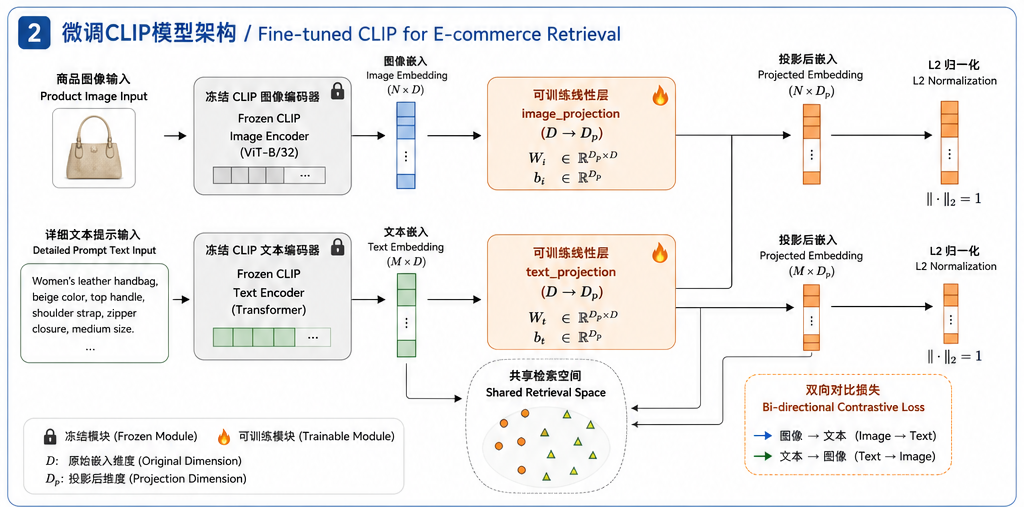
\includegraphics[width=0.72\textwidth]{assets/report_figures/clip微调架构图.png}
    \caption{Linear Probe 微调结构}
    \label{fig:clip-linear}
\end{figure}

\subsection{LoRA 微调}

LoRA 是另一种参数高效微调方法。它同样冻结原始 CLIP 的大部分参数，但不再只调整输出端的线性投影层，而是在模型内部的部分线性层和注意力模块中注入低秩可训练分支。对于原始权重矩阵 $W$，LoRA 不直接更新 $W$，而是使用两个低秩矩阵 $A$ 和 $B$ 学习权重增量：
\begin{equation}
    h = Wx + \frac{\alpha}{r}BAx
\end{equation}

其中 $r$ 为低秩矩阵的秩，$\alpha$ 为缩放系数。与 Linear Probe 只改变最终 embedding 空间不同，LoRA 可以对编码器内部的特征提取过程进行轻量调整，因此理论上具有更强的领域适配能力。本文在 CLIP 文本 Transformer 和视觉 Transformer 的后部 block 中注入 LoRA 模块，使模型在保持输出维度 512 不变的情况下适配 ABO 商品检索任务。

\subsection{向量数据库检索}
在数据规模较小时，可以直接将所有 text embedding 和 image embedding 组成相似度矩阵，并在内存中完成 Top-K 排序。但在真实电商场景中，候选商品数量可能达到百万甚至亿级，直接保存和遍历完整相似度矩阵会带来很高的内存和计算开销。因此，更常见的做法是将商品向量写入向量数据库，并通过近似最近邻检索算法进行高效召回。常见工具包括 ChromaDB、Faiss 等。

本文实验使用 ChromaDB 构建图片向量库。离线阶段，模型先对测试集图片进行编码，并以 \texttt{ProductId\_img} 作为向量 ID 将图片 embedding 写入数据库；在线评估阶段，系统将不同细粒度的文本 prompt 编码为查询向量，再基于余弦距离从图片向量库中检索 Top-K 候选图片。该流程使实验实现与实际商品检索系统的架构更加接近。

\begin{figure}[H]
    \centering
    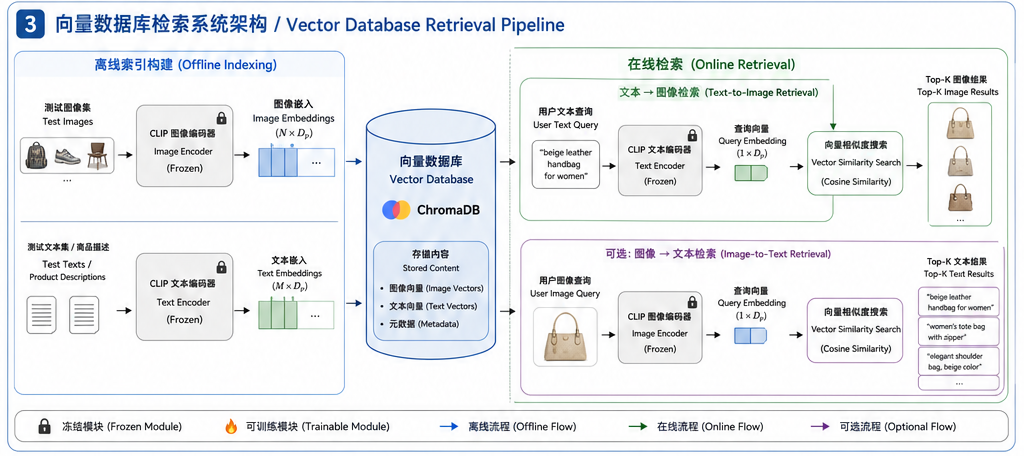
\includegraphics[width=0.76\textwidth]{assets/report_figures/clip向量数据库架构图.png}
    \caption{向量数据库检索流程}
    \label{fig:vector-db}
\end{figure}

\section{实验设置}

\subsection{训练与超参数}

Linear Probe 通过网格搜索选择超参数。考虑到原始 CLIP 与 LoRA 的输出均为 512 维，本文固定 \texttt{embedding\_dim=512}，搜索学习率和温度系数。最终以 \texttt{full} prompt 的 \texttt{Recall@5} 和 \texttt{MRR@5} 作为主要选择依据。

\begin{table}[H]
    \centering
    \caption{最佳 Linear Probe 超参数}
    \label{tab:hyperparams}
    \begin{tabular}{lc}
        \toprule
        \textbf{参数} & \textbf{取值} \\
        \midrule
        学习率 & 0.001 \\
        投影维度 & 512 \\
        温度系数 & 0.07 \\
        训练轮数 & 20 \\
        Early stopping patience & 3 \\
        Batch Size & 128 \\
        \bottomrule
    \end{tabular}
\end{table}

\subsection{评价指标}

本文采用 \texttt{Recall@K}、\texttt{MRR@K} 和 \texttt{NDCG@K} 作为评价指标。

\textbf{Recall@K} 衡量正确图片是否出现在前 $K$ 个候选中：
\begin{equation}
    \mathrm{Recall}@K = \frac{1}{|\mathcal{Q}|}\sum_{q \in \mathcal{Q}} \mathrm{Hit}@K(q)
\end{equation}

\textbf{MRR@K} 衡量正确图片排名倒数的平均值：
\begin{equation}
    \mathrm{MRR}@K = \frac{1}{|\mathcal{Q}|}\sum_{q \in \mathcal{Q}} \mathrm{RR}@K(q)
\end{equation}

\textbf{NDCG@K} 在是否命中的基础上进一步考虑排名位置折损：
\begin{equation}
    \mathrm{NDCG}@K = \frac{1}{|\mathcal{Q}|}\sum_{q \in \mathcal{Q}}
    \frac{\sum_{r=1}^{K}\mathrm{rel}_r(q)/\log_2(r+1)}{\mathrm{IDCG}@K(q)}
\end{equation}

\section{实验结果}

\subsection{Top-5 Prompt 细粒度结果}

\begin{table}[H]
    \centering
    \caption{不同模型在五种 prompt 下的 Top-5 检索结果}
    \label{tab:top5-prompt}
    \resizebox{\textwidth}{!}{
    \begin{tabular}{llccc}
        \toprule
        \textbf{模型} & \textbf{Prompt} & \textbf{Recall@5} & \textbf{MRR@5} & \textbf{NDCG@5} \\
        \midrule
        Original CLIP & type & 0.0482 & 0.0220 & 0.0284 \\
        Original CLIP & material & 0.0688 & 0.0333 & 0.0420 \\
        Original CLIP & brand & 0.0527 & 0.0269 & 0.0332 \\
        Original CLIP & brand\_material & 0.0786 & 0.0359 & 0.0463 \\
        Original CLIP & full & 0.5446 & 0.3601 & 0.4059 \\
        \midrule
        CLIP+Linear Probe & type & 0.0366 & 0.0172 & 0.0219 \\
        CLIP+Linear Probe & material & 0.0741 & 0.0316 & 0.0420 \\
        CLIP+Linear Probe & brand & 0.1080 & 0.0530 & 0.0664 \\
        CLIP+Linear Probe & brand\_material & 0.1357 & 0.0683 & 0.0849 \\
        CLIP+Linear Probe & full & 0.8000 & 0.5970 & 0.6478 \\
        \midrule
        CLIP+LoRA & type & 0.0446 & 0.0215 & 0.0272 \\
        CLIP+LoRA & material & 0.0866 & 0.0431 & 0.0538 \\
        CLIP+LoRA & brand & 0.0893 & 0.0447 & 0.0556 \\
        CLIP+LoRA & brand\_material & 0.1214 & 0.0670 & 0.0805 \\
        CLIP+LoRA & full & \textbf{0.8339} & \textbf{0.6457} & \textbf{0.6929} \\
        \bottomrule
    \end{tabular}}
\end{table}

\subsection{完整标题 Prompt 下的 Top-K 对比}

\begin{table}[H]
    \centering
    \caption{\texttt{full} prompt 下不同 Top-K 的模型对比}
    \label{tab:full-topk}
    \begin{tabular}{llccc}
        \toprule
        \textbf{Top-K} & \textbf{模型} & \textbf{Recall@K} & \textbf{MRR@K} & \textbf{NDCG@K} \\
        \midrule
        5 & Original CLIP & 0.5446 & 0.3601 & 0.4059 \\
        5 & CLIP+Linear Probe & 0.8000 & 0.5970 & 0.6478 \\
        5 & CLIP+LoRA & \textbf{0.8339} & \textbf{0.6457} & \textbf{0.6929} \\
        \midrule
        10 & Original CLIP & 0.6705 & 0.3772 & 0.4470 \\
        10 & CLIP+Linear Probe & 0.8875 & 0.6091 & 0.6766 \\
        10 & CLIP+LoRA & \textbf{0.9009} & \textbf{0.6549} & \textbf{0.7149} \\
        \midrule
        20 & Original CLIP & 0.7705 & 0.3843 & 0.4724 \\
        20 & CLIP+Linear Probe & 0.9330 & 0.6123 & 0.6881 \\
        20 & CLIP+LoRA & \textbf{0.9357} & \textbf{0.6575} & \textbf{0.7238} \\
        \bottomrule
    \end{tabular}
\end{table}

\subsection{微调增益分析}

以 \texttt{full} prompt 的 Top-5 结果为例，Linear Probe 相比原始 CLIP 的 \texttt{Recall@5} 从 $0.5446$ 提升到 $0.8000$，提升 $0.2554$；LoRA 进一步提升到 $0.8339$，相比原始 CLIP 提升 $0.2893$。MRR 和 NDCG 也呈现类似趋势，说明微调不仅提高了是否命中的概率，也改善了正确图片在候选列表中的排序位置。

\begin{table}[H]
    \centering
    \caption{\texttt{full} prompt 下 Top-5 微调增益}
    \label{tab:delta}
    \begin{tabular}{lccc}
        \toprule
        \textbf{对比项} & \textbf{$\Delta$Recall@5} & \textbf{$\Delta$MRR@5} & \textbf{$\Delta$NDCG@5} \\
        \midrule
        Linear Probe $-$ Original CLIP & +0.2554 & +0.2369 & +0.2419 \\
        LoRA $-$ Original CLIP & \textbf{+0.2893} & \textbf{+0.2856} & \textbf{+0.2870} \\
        LoRA $-$ Linear Probe & +0.0339 & +0.0487 & +0.0451 \\
        \bottomrule
    \end{tabular}
\end{table}

\subsection{Linear Probe 投影位置消融实验}

为进一步分析 Linear Probe 中图像侧投影层和文本侧投影层各自的作用，本文补充设计了三组消融实验：\texttt{text+vision} 表示同时在图像编码器和文本编码器输出后加入线性层；\texttt{text only} 表示只在文本侧加入线性层，图像侧保持原始 CLIP embedding；\texttt{vision only} 表示只在图像侧加入线性层，文本侧保持原始 CLIP embedding。三组实验均使用 grid search 得到的最优参数，即学习率 $0.001$、温度系数 $0.07$、训练轮数 $20$，并统一使用 \texttt{full} prompt 进行训练。

\begin{table}[H]
    \centering
    \caption{Linear Probe 投影位置消融实验的 Top-5 结果}
    \label{tab:linear-ablation-top5}
    \resizebox{\textwidth}{!}{
    \begin{tabular}{llccc}
        \toprule
        \textbf{投影方式} & \textbf{Prompt} & \textbf{Recall@5} & \textbf{MRR@5} & \textbf{NDCG@5} \\
        \midrule
        text+vision & type & 0.0348 & 0.0155 & 0.0203 \\
        text+vision & material & 0.0670 & 0.0303 & 0.0393 \\
        text+vision & brand & 0.1018 & 0.0494 & 0.0623 \\
        text+vision & brand\_material & 0.1375 & 0.0702 & 0.0867 \\
        text+vision & full & \textbf{0.7875} & \textbf{0.5902} & \textbf{0.6397} \\
        \midrule
        text only & type & \textbf{0.0429} & 0.0190 & 0.0249 \\
        text only & material & \textbf{0.0777} & \textbf{0.0359} & \textbf{0.0461} \\
        text only & brand & \textbf{0.1089} & \textbf{0.0511} & \textbf{0.0653} \\
        text only & brand\_material & \textbf{0.1402} & \textbf{0.0703} & \textbf{0.0874} \\
        text only & full & 0.7366 & 0.5136 & 0.5693 \\
        \midrule
        vision only & type & 0.0411 & \textbf{0.0198} & \textbf{0.0250} \\
        vision only & material & 0.0741 & 0.0349 & 0.0445 \\
        vision only & brand & 0.0973 & 0.0447 & 0.0576 \\
        vision only & brand\_material & 0.1143 & 0.0586 & 0.0724 \\
        vision only & full & 0.7438 & 0.5219 & 0.5770 \\
        \bottomrule
    \end{tabular}}
\end{table}

\begin{table}[H]
    \centering
    \caption{\texttt{full} prompt 下 Linear Probe 投影位置消融的 Top-K 对比}
    \label{tab:linear-ablation-full-topk}
    \begin{tabular}{llccc}
        \toprule
        \textbf{Top-K} & \textbf{投影方式} & \textbf{Recall@K} & \textbf{MRR@K} & \textbf{NDCG@K} \\
        \midrule
        5 & text+vision & \textbf{0.7875} & \textbf{0.5902} & \textbf{0.6397} \\
        5 & text only & 0.7366 & 0.5136 & 0.5693 \\
        5 & vision only & 0.7438 & 0.5219 & 0.5770 \\
        \midrule
        10 & text+vision & \textbf{0.8777} & \textbf{0.6025} & \textbf{0.6691} \\
        10 & text only & 0.8500 & 0.5287 & 0.6060 \\
        10 & vision only & 0.8554 & 0.5371 & 0.6135 \\
        \midrule
        20 & text+vision & \textbf{0.9384} & \textbf{0.6069} & \textbf{0.6847} \\
        20 & text only & 0.9080 & 0.5330 & 0.6210 \\
        20 & vision only & 0.9205 & 0.5419 & 0.6303 \\
        \bottomrule
    \end{tabular}
\end{table}

\section{结果分析与讨论}

\subsection{Prompt 细粒度影响显著}

从表~\ref{tab:top5-prompt} 可以看出，\texttt{full} prompt 明显优于其它四类属性拼接 prompt。以原始 CLIP 为例，\texttt{type} 的 \texttt{Recall@5} 仅为 $0.0482$，而 \texttt{full} prompt 达到 $0.5446$。这说明在 ABO 商品检索任务中，完整标题包含了更丰富的商品名称、款式、规格和用途信息，能更有效地区分同一类别中的相似商品。

\subsection{品牌和材质有帮助，但不足以替代标题}

加入品牌和材质后，prompt 表现通常优于只使用类别。例如 Linear Probe 的 \texttt{brand\_material} 在 Top-5 下达到 $0.1357$，高于 \texttt{type} 的 $0.0366$。但相比 \texttt{full} prompt 的 $0.8000$ 仍有巨大差距，说明品牌和材质只能提供部分判别信息，而商品标题仍是最有效的文本来源。

\subsection{LoRA 在完整标题条件下表现最佳}

LoRA 在 \texttt{full} prompt 下取得所有模型中的最佳结果，Top-5、Top-10、Top-20 的 Recall 分别为 $0.8339$、$0.9009$、$0.9357$。这说明 LoRA 能在保持 CLIP 原有语义空间的基础上进一步适配 ABO 商品域，尤其有利于完整商品标题这种信息密度较高的查询形式。

\subsection{Linear Probe 投影位置的影响}

从表~\ref{tab:linear-ablation-top5} 可以看出，Linear Probe 的投影位置对不同类型 prompt 的影响并不完全相同。对于 \texttt{type}、\texttt{material}、\texttt{brand} 和 \texttt{brand\_material} 等属性型 prompt，\texttt{text only} 通常优于 \texttt{vision only}，例如在 \texttt{brand\_material} prompt 下，\texttt{text only} 的 \texttt{Recall@5} 为 $0.1402$，高于 \texttt{vision only} 的 $0.1143$。这与本文的预期基本一致：由于当前任务是 text-to-image 检索，查询端来自文本 prompt，因此只调整文本侧 embedding 可以更直接地改善不同细粒度 prompt 与图片向量之间的对齐关系。

但在 \texttt{full} prompt 下，最优结果来自 \texttt{text+vision} 双侧投影。表~\ref{tab:linear-ablation-full-topk} 显示，\texttt{text+vision} 在 Top-5、Top-10 和 Top-20 下均取得最高的 Recall、MRR 和 NDCG。这说明当 prompt 包含完整商品标题时，文本信息已经足够丰富，仅调整文本侧虽然能够适配查询表达，但同时调整图像侧和文本侧可以进一步重塑两种模态的共同 embedding 空间，从而获得更好的整体排序质量。因此，消融实验表明：对于较粗粒度属性 prompt，文本侧投影更关键；而对于信息量更大的完整标题 prompt，双侧投影仍然是更稳定、更有效的选择。

\subsection{Top-K 增大时 Recall 稳定上升}

从表~\ref{tab:full-topk} 可以看到，随着 $K$ 从 5 增加到 20，三类模型的 Recall 均稳定上升。例如 LoRA 的 Recall 从 $0.8339$ 增至 $0.9357$。MRR 和 NDCG 的提升幅度相对较小，这是因为它们更关注正确结果是否排在靠前位置；如果正确图片主要从第 6 到第 20 位被补充命中，Recall 会明显上升，而 MRR/NDCG 增益会较温和。

\section{不足与改进方向}

本实验仍存在以下不足：
\begin{enumerate}[leftmargin=2em, itemsep=0pt]
    \item \textbf{类别内部存在视觉近似商品。} 例如同类家具、地毯、墙饰往往外观相近，模型可能返回语义相关但并非同一商品的图片。
    \item \textbf{部分字段存在噪声。} 颜色字段中存在 \texttt{Unknown Color}、\texttt{Multi} 等不稳定值，因此本实验未使用颜色构造 prompt。未来可通过规则清洗或人工映射获得更可靠的颜色描述。
    \item \textbf{完整标题带来强语义优势。} \texttt{full} prompt 的性能远高于属性 prompt，说明实验结果很大程度依赖商品标题质量。后续可以进一步比较标题截断、属性重写和自然语言改写对检索性能的影响。
    \item \textbf{当前仅评测 text-to-image。} 后续可以补充 image-to-text 或 image-to-image 方向，使检索系统评估更加完整。
\end{enumerate}

\section{结论}

本文基于 ABO 商品子集构建了一个 CLIP 电商图文检索实验系统，比较了原始 CLIP、Linear Probe 和 LoRA 三种模型，并系统分析了五种 prompt 细粒度对 text-to-image 检索性能的影响。实验结果表明，完整商品标题 prompt 是影响检索性能的关键因素；在此基础上，轻量微调能够显著提升模型在商品域上的匹配能力。其中 LoRA 在 \texttt{full} prompt 下取得最佳结果，\texttt{Recall@5}、\texttt{MRR@5} 和 \texttt{NDCG@5} 分别达到 $0.8339$、$0.6457$ 和 $0.6929$。此外，Linear Probe 消融实验进一步表明，文本侧投影对属性型 prompt 更关键，而在完整标题 prompt 下，同时调整文本侧和图像侧投影能够获得更稳定的最优结果。

总体来看，CLIP 具备较强的电商商品跨模态检索能力，而面向具体商品域的轻量微调和高质量 prompt 构造是进一步提升性能的关键。

\end{document}
